\subsection{İstanbul İslam Bilim ve Teknoloji Tarihi Müzesi}
\indent\indent İstanbul İslam Bilim ve Teknoloji Tarihi Müzesi, iki kattan müteşekkil olup; astronomi, zaman ve saatler, savaş aletleri, madenler, matematik ve geometri, mimari ve şehircilik, kimya, optik gibi çeşitli sergiler ihtiva etmektedir. Aşağıda, daha öne çıkan astronomi, zaman ve saat ve savaş aletleri sergilerine değineceğiz.
\subsubsection{Astronomi Sergisi}
\indent\indent Ağırlıklı olarak sekstantların va gözlemevlerinin minyatürlerinin sergilnediği kısımıdır. Sekstant, yerküre üzerinde bulunulan yerin enlemini ve boylamını belirlemek amacıyla, bir gök cismiyle ufuk düzlemi arasındaki açısal mesafeyi ölçmekte kullanılan optik seyir cihazı.\cite{sekstant} 60 derecelik yaya sahip olduğu için Latincedeki sextus(altıda bir, altıncı) kelimesinden hareketle sextant adı verilmiştir. Sekstantla açı ölçmek için, gemici sekstant dürbününden, ufuk hattına bakar. Gemici, gemi güvertesinde dik olarak durduğu ve gemiyle beraber sallandığı için ölçülecek açı hiç değişmez. Güneşin aynalardan yansıyan görüntüsü tam ufuk hattıyla çakıştığı an sekstant açısı okunur.\newline
\indent Bu kısımda, 903 yılında doğmuş Abdurrahman es-Sufî'nin tasavvur ettiği gök kürenin de bir örneği incelenebilir. Abdurrahman es-Sûfî, sabit yıldızların sistematik incelenmesi ve kataloglanmasında Batlamyus’tan sonra en önemli isimlerden biridir. Kitâbü Ṣuveri’l-kevâkibi’s̱-s̱âbite adlı eserinde kırk sekiz yıldız takımını ayrıntılı biçimde ele alarak yıldızların konum, parlaklık ve renk bilgilerini açıklamış, Batlamyus’un terminolojisini Arapçaya kazandırmıştır. Es-Sûfî’nin tanımladığı terimlerden doksan dördü modern astronomi literatüründe hâlen kullanılmaktadır.\cite{dia_8}\newline
\begin{figure}[H]
    \centering
    \subfigure[Sekstantlar]{
        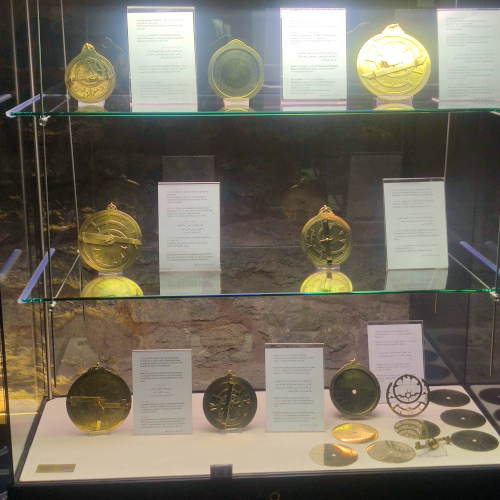
\includegraphics[width=0.55\textwidth,height=0.45\textheight]{assets/sekstant.jpg}
    }
    \hfill
    \subfigure[Abdurrahman es-Sufî'nin Gök Küresi]{
        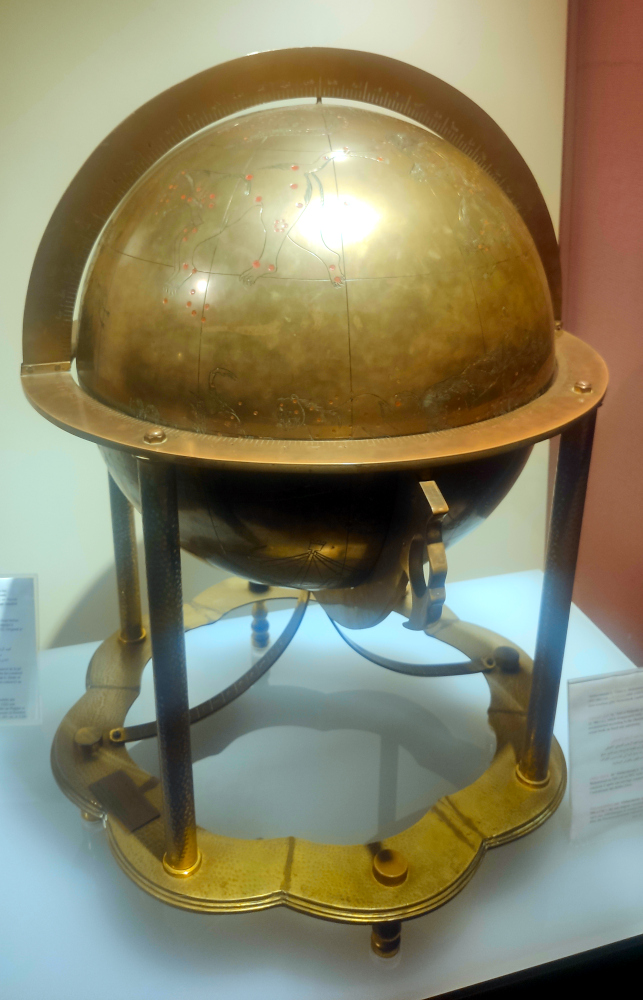
\includegraphics[width=0.4\textwidth,height=0.45\textheight]{assets/sphere.jpg}
    }
    \caption{Astronomi ile ilgili eserler}
\end{figure}
\subsection{Zaman ve Saat}
\indent\indent Bu bölümde, Arap ve İslam bilim insanlarının zamanı ölçmek için ürettiği saatlerin prototiplerini incelemek mümkün. Müzenin en dikkat çekici eserlerinde birisi de Fas Ḳaraviyyīn Camii’nde bulunan su saati modelidir. Bu model, günü 24 saate bölen, günümüze ulaşmış en eski su saatidir. Her saatin 4er dakikaya(yani 15 bölüme) bölümlendiği bir saat kadranında tasarlanmıştır. Her dört dakikada küçük bir küre, her bir saatte ise büyük bir küre 24 pirinç kaseden birisine düşer ve bir ses oluşturur. 24 saat zarfında toplam 360 küçük ve 24 büyük küre kaselere, oradan da bir toplama haznesine düşer. Akustik sinyallere ilaveten, her saat başı, geçen zamana dair genel bir bakış veren ve uzaktan da görülebilen ahşap kapılardan birisi kapanır. Düzenek, dökülen su aracılığıyla harekete geçirilir. Bu su, ipli makaralar vasıtasıyla işleyen bütün kısımların bağlantıda olduğu bir şamandrayı aşağı indirir. Düzenli akış, tam olarak basınç ayarlayan bir cihaz vasıtasıyla sağlanır.\newline
\begin{figure}[H]
    \centering
    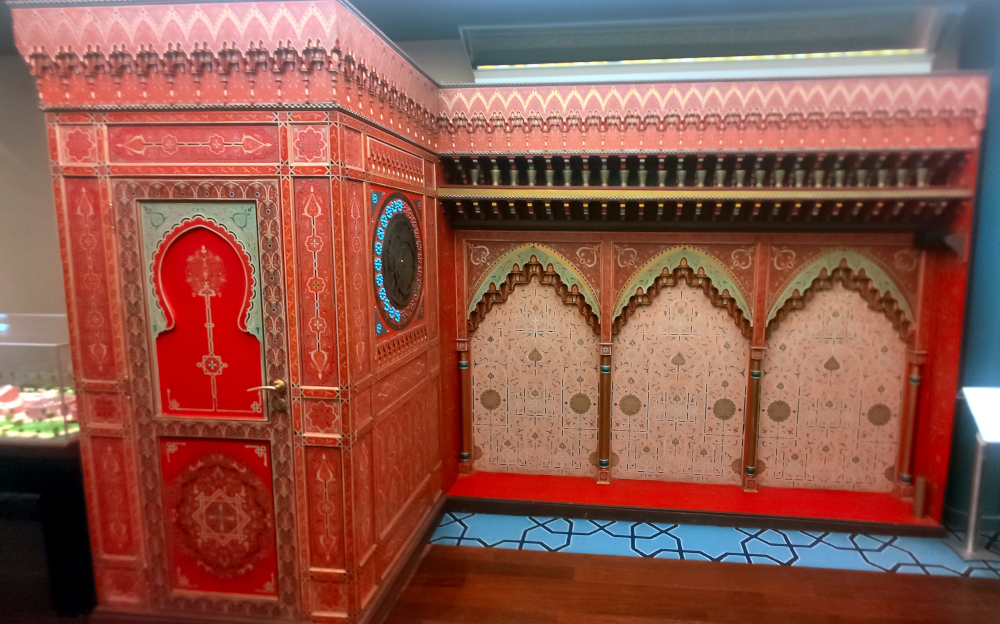
\includegraphics[width=0.95\linewidth]{assets/water_clock.jpg}
    \caption{Fas Su Saati}
\end{figure}
\newpage
\subsection{Savaş Aletleri}
\begin{wrapfigure}{r}{0.2\textwidth}
    \centering
    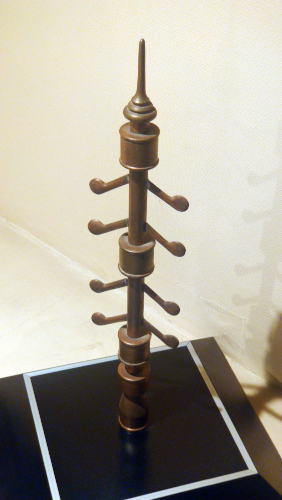
\includegraphics[width=0.2\textwidth]{assets/lageri.jpg}
    \caption{Lagari Hasan Çelebi'nin Roketi}
\end{wrapfigure}
\indent\indent Türk ve İslam devletlerinin yaptığı savaşlarda kullanılan aletlerin sergilendiği bölüm. Ağırlıklı olarak kuşatma aletlerini ve mancınık modellerini ihtiva etmektedir. Bu kısımda en ilgi çekici eser ise, Lagari Hasan Çelebi'nin tasarladığı roket modelidir. Lagari Hasan Çelebi, 1632 ya da 1633 yılında Sarayburnu'nda IV.Murad'ın da hazır bulunduğu denemede, kendisini tasarladığı rokete bağlatmış olduğu halde roketi ateşletmiştir. 300 metre kadar yükseldikten sonra barutu biten roket serbest düşüşe geçmiş, Lagari Hasan Çelebi kollarına bağladığı kanatları açarak yumuşak iniş yapmıştır. Hikayenin doğruluğu oldukca şüphelidir, çünkü Lagari Hasan Çelebi'yi anlatan tek kaynak Evliya Çelebi'nin \textit{Seyahatname} isimle eseridir.\newline
